\titre{Principes généraux :}
\begin{itemize}
	\item Découper le projet en phases, étapes et taches $\rightarrow$ plus on découpe, plus on avance
	\item Pour chacune : 
	\begin{itemize}
		\item Date de début au plus tôt
		\item Date de fin au plus tôt
		\item Date de début au plus tard
		\item Date de fin au plus tard
		\item $\rightarrow$ La différence entre date de début au plus tôt et de début au plus tard s'appelle la \titre{marge} de la tache.
	\end{itemize}
\end{itemize}

\titre{PERT :} Program Evaluation and Review Technique 
\begin{itemize}
	\item Permet de visualiser la \titre{dépendance des tâches} et de procéder à leur \titre{ordonnancement} $\rightarrow$ graphe de dépendance des tâches.
	\item Permet de mener un projet dans les contraintes de temps et d'identifier les \titre{tâches critiques} (doit commencer au plus tard à la date ou elle peut commencer au plus tôt) qui conditionnent la \titre{durée minimale du projet} \\
	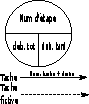
\includegraphics[width=100px]{Images/fig1.pdf} 
\end{itemize}

\titre{Date au plus tôt :} Parcours du diagramme de gauche à droite et calcul du temps du plus long chemin menant du début du projet à cette tâche \\

\titre{Date de début au plus tard :} Parcours du diagramme de droite à gauche, en commençant à la durée totale du projet puis on soustrait à chaque étape la durée de la tâche. \\

\titre{Exemple :}
\begin{enumerate}
	\item Préparer le menu (30min)
	\item Acheter les ingrédients (90min)
	\item Préparer l'apéritif (30min)
	\item Nettoyer la table (10min)
	\item Mettre la table (10min)
	\item Préparer les ingrédients (30min)
	\item Cuisiner les plats (60min)
	\item Servir le repas (10min)
\end{enumerate}
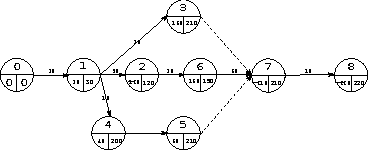
\includegraphics[width=300px]{Images/fig2.pdf}
\\

\titre{Gantt :} 
\begin{enumerate}
	\item Abscisse : temps
	\item Ordonnée : différentes tâches ou lots
	\item Durée d'exécution d'une tâche = barre horizontale
	\item Liens de dépendance entre les tâches : flèche
\end{enumerate}

\titre{Construction :}
\begin{enumerate}
	\item Définir la liste des tâches avec leurs dépendances et leur durée, puis la liste des ressources affectées à chacune des tâches
	\item Placer les tâches à effectuer dans le diagramme de Gantt dans l'ordre défini par leur priorité et en fonction des ressources encore disponibles
	\item Placer des jalons (tâches importantes à temps presque nul et indispensables (ex : présentation du cahier des charges).
\end{enumerate}

\titre{Les règles les plus courantes d'affectation des ressources sont :}
\begin{enumerate}
	\item Priorité à la réalisation des fabrications dont la date de livraison est la plus rapprochée
	\item Priorité à la première commande arrivée
	\item Priorité aux fabrications dont la durée totale est la plus courte (ou l'inverse selon la criticité)
	\item Priorité aux fabrications qui utilisent le moins de ressources critiques
	\item Priorité aux fabrications qui disposent du minimum de marge globale
\end{enumerate}

\titre{Avancement :}
\begin{enumerate}
	\item Barre de durée remplie proportionnellement à son degré d'accomplissement
	\item Ligne verticale sur la date de jour : tâches accomplies à gauche, tâches non commencées à droite, tâches en cours traversent la ligne
	\item Les jalons permettent de scinder le projet en phases clairement identifiées.
\end{enumerate}
